\chapter{Analysis}

In this chapter, we will be doing problem analysis. We will dive deeper into the problem we intend to fix, and why we think it is a problem in the first place. We will discuss various existing approaches that already solve part of the problem, and why these are great efforts. We finish by discussing why believe that the existing approaches fall short of what we aim to achieve.

\section{Problem Definition}

Now is as good a time as any to outline the problem at hand more concretely. Simply put, we aim to present computer programs at different abstraction levels, without losing the underlying ideas. This can be - and traditionally also has been - done ``manually'' by the program authors. For instance: writing a computer program, testing it, and later rewriting the source code to some sort of pseudocode. We believe that this process could be automated to some extent, to the benefit of all involved. \hfill \\

There are several use cases where displaying source code with an alternative representation could be useful. Mainly within education, where the goal is to teach students concepts in an agonstic way. However, it could also be used by researchers exchanging ideas, across preferred programming languages. \hfill \\

Already in the 80's Clements et al. predicted that computers would be an integral part of the classroom~\cite{clements1984effects}. Slowly but surely also the art of computer programming has been introduced into school curriculums, at a younger and younger age. \hfill \\

Instructing 10-year-olds in complex concepts like pointers and multi-threading may not be the most effective use of time. However, there is value in familiarizing them with computer programming, which is a fundamental aspect of our increasingly digital world. \\

If the teacher is to transpile her code to flowcharts, it offers a visual approach to understanding programming concepts. Consequently, the whole classroom can focus on the underlying logic than on the syntactic quirks of the teacher's preferred programming language. \hfill \\ % Aditionally, the flowcharts could be fairly easy to recreate in an imperative programming language

This is also the case when teaching computer programs at a higher level, like university. Opting for pseudocode instead of a specific programming language levels the playing field, as well as helping students coming from a mathematical background. \hfill \\

Lastly, researchers might wish to exchange ideas despite using different programming languages. Just like every animal in the kingdom can be called upon in latin, every idea can be presented more neutrally with pseudocode. \hfill \\

\forsup{For tynt eller ok?}

In the context of our problem, and the remainder of this thesis, we choose to also treat flowcharts as a form of pseudocode. As such, we have to make a distinction between flowcharts and traditional pseudocode, which more closely resembles source code. From now, when discussing both forms in the same context, traditional pseudocode will be referred to as \textbf{Text based pseudocode} (TBP) and flowcharts as \textbf{Image based pseudocode} (IBP).

\section{Comparing source code with TBP and IBP}

In this section we aim to show how the same computer program can be presented in three different levels of abstraction. The first one will be source code written in a popular programming language, while the latter two will be TBP and IBP. \\

The program in question \forsup{beskrivelse programmet. Mulig bucket sort eller en tre-algoritme kan egne seg her.}

Listing ?? shows the program written in the programming language Go/Java. Figure ?? and Figure ?? show the same program, but with TBP and IBP, respectively. \hfill \\

The main similarity between the source code and the TBP is that both versions resemble an executable program. People familiar with programming will likely understand the logic conveyed by the pseudocode, even if they have no prior experience with the Algorithm2e library. Both versions present each instruction as sequential lines, and employ syntax like \texttt{if} and \texttt{else}. \forsup{Forklare likhetene nærmere?}

The main difference is the format. For one, the TBP version describes the input and output, which allows us to have rather succinct parameter names. In the Go/Java example, even though the parameter names are explanatory, we cannot always be 100\% sure about how the author intends for them to be applied. This is not an issue with TBP. \\

Another thing to notice is the difference in notation. While in Go/Java we have to write terms like \texttt{!=} and \texttt{ceil(x)}, TBP allows us to use more precise mathematical notation like \texttt{$\neq$} and \texttt{$\lceil$x$\rceil$}. \\

Additionally, since the TBP is intentionally not executable, we allow ourselves to omit implementation specific details that are not crucial to understand the program's logic. This makes for a more concise presentation, minimising the chance of confusion by whoever is trying to understand the program. \\

The same can be said for the IBP version, which does not particularly resemble the original source program. In appearance, they are on very different abstraction levels. Whereas the code is written in sequential lines, the flowchart shows colourful shapes wandering off in different directions. \\

The spacing and colourfulness of IBP can make it easier to isolate parts of the program, and to see more precisely how each part works individually. It also makes it easier to follow each path of the program, compared to the Go/Java program, where the order of function calls and scoping of if-statements can confuse even more seasoned programmers. \\

The notation stays much the same, but since the flowcharts are not executable, we can again opt for more precise mathematical notation to describe expressions, and exclude static properties like types.

\section{Related work}

This section will cover selected related software, that has already solved parts of the problem in its own right. We have separated the section into two further subsections, to analyse contributions related to TBP and IBP individually.

\subsection{Source code to TBP}

Despite TBP being used in so many text books, online courses and published papers, the amount of source code-to-pseudocode-editors currently available on the internet is anything but overwhelming. Additionally, there is no undisputed choice that is commonly used. There are, however, a couple of candidates who stick out if we look closely enough.

\subsubsection{Naive approach}

The naive approach would be to do this manually. Perhaps the wording is too harsh, but in this context, \texttt{naive} really just corresponds to \texttt{manual}. By manually writing our own pseudocode, we are void of any restrictions, and can do it just the way we like. \\

The downside is the extra effort of writing both the original algorithm, in addition to spending time on writing the pseudocode. Doing it this way means we also have to maintain both versions manually. We might change our source code but forget to update the pseudocode, and we are likely to spend some time on trying to abstract the pseudocode in the first place.

\subsubsection{Pseudogen}

The Psuedogen transpiler is currently designed to work with a subset of the Python programming language~\cite{DBLP:conf/kbse/OdaFNHSTN15}. The output target is purely natural language, precisely like majority of this thesis. As mentioned in Section 2.1.1, the tool is developed using statistical machine translation. This is a technique of translating from one language to another based on statistical models, and is generally used to translate between natural languages (which makes Python such a natural choice). \hfill \\

Despite being a programming language notoriously known for using plain English where many other programming languages use more technical notation ($and$ instead of $\&\&$, $or$ instead of $||$ etc.), Python still bears the mark of being a programming language. People unfamiliar with programming and/or mathematics might still struggle to understand some of the more technical aspects of its syntax. \hfill \\

Figure 3.1 shows an example taken from the initial 2015 paper where Pseudogen was first presented. It displays Python source code on the left, and pseudocode on the right. The program in question is an algorithm that solves the \textbf{FizzBuzz} problem, commonly presented in entry level interview settings and beginner programming exercises. \hfill \\

\begin{figure}[ht]
    \centering
    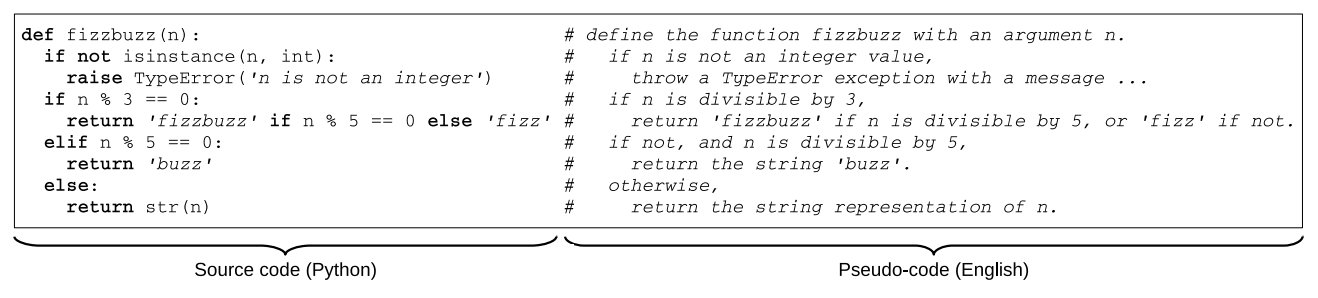
\includegraphics[scale=0.52]{assets/odaetal.png}
    \caption{Example of source code written in Python and corresponding pseudocode created by Pseudogen}
    \label{fig:odaetal}
\end{figure}

What the examples in the 2015 paper, as well as a video on their website show, is really a line-for-line translation to English. \footnote{The Pseudogen website can be found at https://ahclab.naist.jp/pseudogen/} This could be desired in cases where the business people on the team are particularly curious about what the product is really doing under the hood (without having to refactor the code base to Cobol). \\

However, since Pseudogen will translate each line in a servile manner, all error handling is translated too. Listing 3.1 shows some error handling in Python, and Listing 3.2 shows the result from transpiling it with Pseudogen. The result is overwhelmingly verbose, which also defeats much of the point with Python, whose syntax tends to be elegant and succinct, already closely resembling natural language. \\ \\

% Obs, lagt inn ekstra newline over!

\begin{lstlisting}[caption={Error handling in Python}, captionpos=b]
except ValueError as e:
    print(e)
\end{lstlisting}

\begin{lstlisting}[caption={The result of transpiling the code in Listing ?? with Pseudogen}, captionpos=b]
# If ValueError, renamed to e, exception is caught.
    # Call the function print with an argument e.
\end{lstlisting}

Another example is visible in Listing 3.3 and Listing 3.4, where list comprehension has been translated very literally. It is plausible to assume people with backgrounds in academia might favour the Python version to the transpiled one, as it closely resembles how we would write set comprehension in mathematics. \hfill \\

\begin{lstlisting}[caption={A list comprehension of applying f(n) to integers in the range -10 to 10, and placing the results in a list}, captionpos=b]
a = [f(n) for n in range(-10, 10)]
\end{lstlisting}

\begin{lstlisting}[caption={The result of transpiling the code in Listing ?? with Pseudogen}, captionpos=b]
# Call the function f with an argument n for every
  n in range of integers from range 10 negative
  integer 10, substitute the result for a
\end{lstlisting}

It is clear that the target audience for Pseudogen's output formats must be people with little to no experience with reading/writing code. It seems like an excellent tool for translating Python to English, and shows that something like this is indeed possible. However, Psnodig's intended target audience is broader, and thus we believe Pseudogen alone is not enough to solve the problem we are dealing with.

\subsubsection{PseudoEditor}

\forsup{Har ikke fått denne til å funke enda! Synes ikke den gir ikke mening i det hele tatt. Gjerne sjekk den ut på \url{https://pseudoeditor.com/app/}. Selv ikke å poste eksemplet fra \url{https://pseudoeditor.com/guides/merge-sort} fungerer..}

\forsup{Føler derimot at jeg bør ha flere enn ett eksempel på 'source code -> pseudocode'. Eller?}

\subsection{Source code to IBP}

Even though there is research arguing for the good effects of flowcharts in computer science, there have been few documented efforts towards developing a tool that can effectively translate source code to flowcharts. However, there does exist some software that lets us write flowcharts through a DSL, and we will look at two of them.

\subsubsection{Naive approach}

Yet again, calling it a naive approach might not be entirely accurate, but manually translating our code to flowcharts does introduce some intricacies. For one, like with TBP, we have to maintain both versions, and if we change too much of our main idea, then the time spent on making the IBP version is - to a certain extent - wasted. \\

Another flaw is that we have to spend time thinking about how the flowchart should look like, which parts could and should be abstracted, how they should be presented instead (or if they should be removed altogether) etc. Which colours should the frames have? How should the arrows look? Which font should be used? By using an automated tool, we do not have to worry about details unrelated to the actual program logic. \\

The perk of doing it this way, however, is that we can do it entirely our way. We can choose which tools we want to use, and if we are already proficient in making flowcharts based on source code, then this actually seems like a natural choice. If we also like spending time on details like colours, fonts, shapes etc., then at least the naive approach does not limit our creativity in any way. \\

\forsup{Jeg føler egentlig at det er naturlig å starte med det positive, og avslutte med det negative?}

\subsubsection{Code2Flow}

Code2Flow is a tool that lets us create flowcharts with natural language, decorated with a C-inspired syntax. Their website states that we might get away with pasting syntactically correct C programs, but that this is purely incidental. This goes to show that the Code2Flow team have indeed developed a DSL with their own syntax. \\

Flowcharts created with Code2Flow have a few, consistent colours to differentiate parts of their corresponding programs. Start- and end expressions are displayed as red ovals, while all remaining expressions are displayed as blue rectangles. Conditionals, loops and match statements are displayed with red rhombuses, and comments are displayed with orange rectangles. \\

\begin{lstlisting}[caption={A Code2Flow program}, captionpos=b]
First expression;
Another expression;
if (conditional) {
  expression 1;
} else {
  expression 2; // Random comment
}
Last expression;
\end{lstlisting}

Listing 3.5 shows a program written with Code2Flow, and Figure 3.2 shows the corresponding flowchart. As we can see, syntactically correct expressions are just any combination of UTF-8 characters. Thus, we have no way to test a Code2Flow program. In fact, Code2Flow will \textit{never} let us know about syntactic errors, and will \textit{always} try to construct whatever flowchart it can. \\

\begin{figure}[ht]
    \centering
    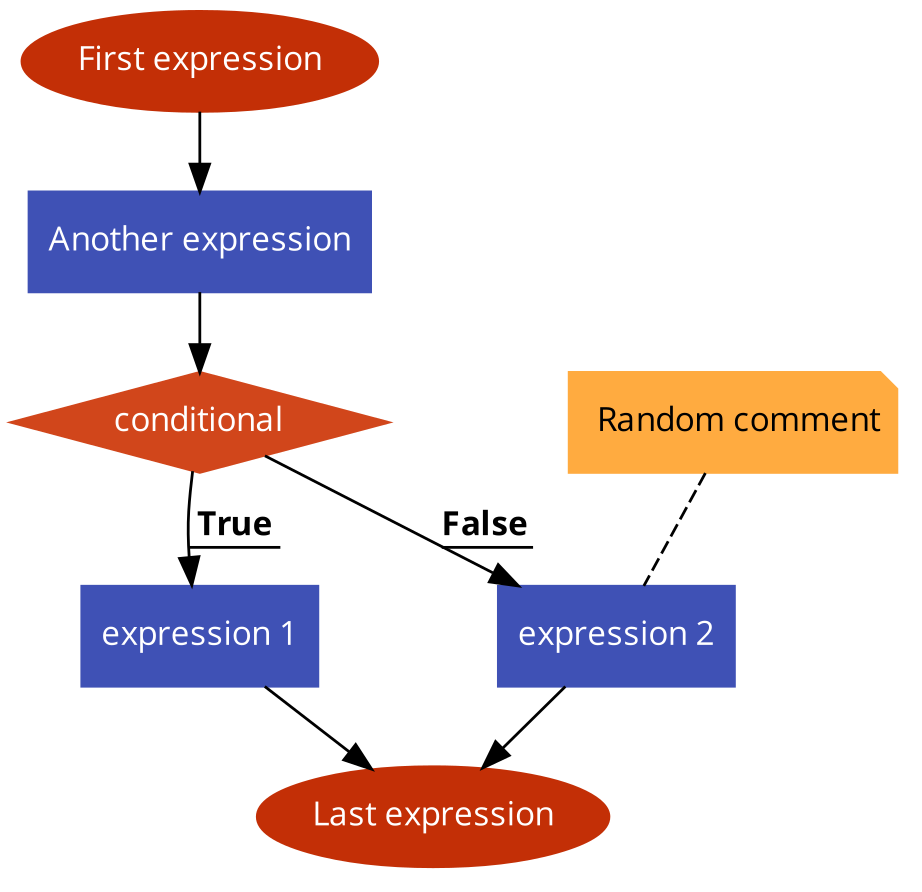
\includegraphics[scale=0.2]{assets/code2flow_example.png}
    \caption{The resulting flowchart from transpiling the Code2Flow code in Listing 3.5}
    \label{fig:code2flow}
\end{figure}

If our C program inadvertently creates a ``correct'' flowchart, we can use a C compiler to test said program on the side. However, we must now maintain both versions, and changes to the C program are not guaranteed to successfully transpile to a new flowchart.

\subsubsection{Mermaid.js}

Mermaid.js is a DSL for rendering diagrams (including flowcharts) from a Markdown-inspired syntax. Even though we can construct many different diagrams with Mermaid.js, we will focus on the flowcharts. \\

Like Code2Flow, they also render flowcharts in real time. However, Mermaid.js will warn us about syntax errors, and only re-render syntactically correct programs. \\

To write a Mermaid.js flowchart, our program must start with \texttt{flowchart TD}. Nodes can come in many different shapes, and are denoted by the types of brackets they use. For instance, \texttt{Node[ ]} displays a rectangle, \texttt{Node(( ))} displays a circle, and \texttt{Node\{ \}} displays a rhombus. Edges also come in many shapes. \texttt{-->} displays an arrow, \texttt{---} displays a simple link, and \texttt{-.->} displays a dotted arrow. \hfill \\

We can also have add text, by writing it either inside the brackets, like \texttt{Node[text]}. Arrows can also include text by breaking them up into two parts, like \texttt{-- text -->}.\footnote{The full documentation can be found at~\url{https://mermaid.js.org/syntax/flowchart.html}} \\

\begin{lstlisting}[caption={A mermaid.js program}, captionpos=b]
flowchart TD
    A([First expression])
        --> B[Another expression]
    B --> C{contidional}
    C -- True --> D[Expression 1]
    C -- False --> E[Expression 2]
        %% Random comment
    D --> F([Last expression])
    E --> F
\end{lstlisting}

Just like with Code2Flow, the text inside these nodes can be anything. Listing 3.5 shows a program written with Mermaid.js, and Figure 3.3 shows the corresponding flowchart. Contrary to Code2Flow, comments are ignored by the parser, and solely exist to aid the programmer. They must also be on their own lines. \\

\begin{figure}[ht]
    \centering
    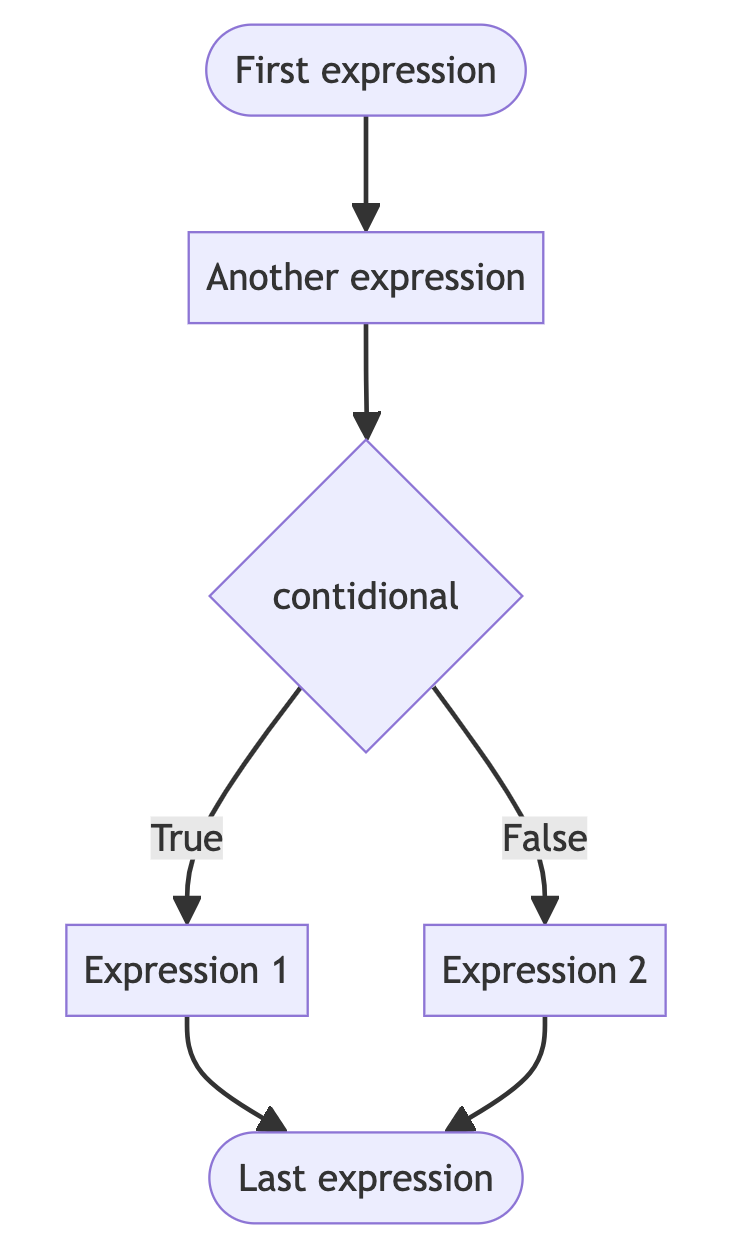
\includegraphics[scale=.5]{assets/mermaidjs.png}
    \caption{The resulting flowchart from transpiling the Mermaid.js code in Listing 3.6}
    \label{fig:code2flow}
\end{figure}

The biggest drawback of Mermaid.js is that the syntax is very different from any programming language. This means pasting our source code will not yield any result, and we have to carefully translate our code every time. This means that it is fully our responsability to maintain the abstraction level we want. Like Code2Flow, Mermaid.js has no way of letting us test the code either.
